\documentclass[11pt,]{article}
\usepackage{lmodern}
\usepackage{amssymb,amsmath}
\usepackage{ifxetex,ifluatex}
\usepackage{fixltx2e} % provides \textsubscript
\ifnum 0\ifxetex 1\fi\ifluatex 1\fi=0 % if pdftex
  \usepackage[T1]{fontenc}
  \usepackage[utf8]{inputenc}
\else % if luatex or xelatex
  \ifxetex
    % \usepackage{mathspec}
    \usepackage{xltxtra,xunicode}
  \else
    \usepackage{fontspec}
  \fi
  \defaultfontfeatures{Mapping=tex-text,Scale=MatchLowercase}
  \newcommand{\euro}{€}
\fi
% use upquote if available, for straight quotes in verbatim environments
\IfFileExists{upquote.sty}{\usepackage{upquote}}{}
% use microtype if available
\IfFileExists{microtype.sty}{%
\usepackage{microtype}
\UseMicrotypeSet[protrusion]{basicmath} % disable protrusion for tt fonts
}{}
\usepackage[top=0.5in, bottom=.4in, left = 1in, right=1in, includeheadfoot]{geometry}
\usepackage{color}
\usepackage{fancyvrb}
\newcommand{\VerbBar}{|}
\newcommand{\VERB}{\Verb[commandchars=\\\{\}]}
\DefineVerbatimEnvironment{Highlighting}{Verbatim}{commandchars=\\\{\}}
% Add ',fontsize=\small' for more characters per line
\usepackage{framed}
\definecolor{shadecolor}{RGB}{248,248,248}
\newenvironment{Shaded}{\begin{snugshade}}{\end{snugshade}}
\newcommand{\KeywordTok}[1]{\textcolor[rgb]{0.13,0.29,0.53}{\textbf{#1}}}
\newcommand{\DataTypeTok}[1]{\textcolor[rgb]{0.13,0.29,0.53}{#1}}
\newcommand{\DecValTok}[1]{\textcolor[rgb]{0.00,0.00,0.81}{#1}}
\newcommand{\BaseNTok}[1]{\textcolor[rgb]{0.00,0.00,0.81}{#1}}
\newcommand{\FloatTok}[1]{\textcolor[rgb]{0.00,0.00,0.81}{#1}}
\newcommand{\ConstantTok}[1]{\textcolor[rgb]{0.00,0.00,0.00}{#1}}
\newcommand{\CharTok}[1]{\textcolor[rgb]{0.31,0.60,0.02}{#1}}
\newcommand{\SpecialCharTok}[1]{\textcolor[rgb]{0.00,0.00,0.00}{#1}}
\newcommand{\StringTok}[1]{\textcolor[rgb]{0.31,0.60,0.02}{#1}}
\newcommand{\VerbatimStringTok}[1]{\textcolor[rgb]{0.31,0.60,0.02}{#1}}
\newcommand{\SpecialStringTok}[1]{\textcolor[rgb]{0.31,0.60,0.02}{#1}}
\newcommand{\ImportTok}[1]{#1}
\newcommand{\CommentTok}[1]{\textcolor[rgb]{0.56,0.35,0.01}{\textit{#1}}}
\newcommand{\DocumentationTok}[1]{\textcolor[rgb]{0.56,0.35,0.01}{\textbf{\textit{#1}}}}
\newcommand{\AnnotationTok}[1]{\textcolor[rgb]{0.56,0.35,0.01}{\textbf{\textit{#1}}}}
\newcommand{\CommentVarTok}[1]{\textcolor[rgb]{0.56,0.35,0.01}{\textbf{\textit{#1}}}}
\newcommand{\OtherTok}[1]{\textcolor[rgb]{0.56,0.35,0.01}{#1}}
\newcommand{\FunctionTok}[1]{\textcolor[rgb]{0.00,0.00,0.00}{#1}}
\newcommand{\VariableTok}[1]{\textcolor[rgb]{0.00,0.00,0.00}{#1}}
\newcommand{\ControlFlowTok}[1]{\textcolor[rgb]{0.13,0.29,0.53}{\textbf{#1}}}
\newcommand{\OperatorTok}[1]{\textcolor[rgb]{0.81,0.36,0.00}{\textbf{#1}}}
\newcommand{\BuiltInTok}[1]{#1}
\newcommand{\ExtensionTok}[1]{#1}
\newcommand{\PreprocessorTok}[1]{\textcolor[rgb]{0.56,0.35,0.01}{\textit{#1}}}
\newcommand{\AttributeTok}[1]{\textcolor[rgb]{0.77,0.63,0.00}{#1}}
\newcommand{\RegionMarkerTok}[1]{#1}
\newcommand{\InformationTok}[1]{\textcolor[rgb]{0.56,0.35,0.01}{\textbf{\textit{#1}}}}
\newcommand{\WarningTok}[1]{\textcolor[rgb]{0.56,0.35,0.01}{\textbf{\textit{#1}}}}
\newcommand{\AlertTok}[1]{\textcolor[rgb]{0.94,0.16,0.16}{#1}}
\newcommand{\ErrorTok}[1]{\textcolor[rgb]{0.64,0.00,0.00}{\textbf{#1}}}
\newcommand{\NormalTok}[1]{#1}
\usepackage{longtable,booktabs}
\usepackage{graphicx}
\makeatletter
\def\maxwidth{\ifdim\Gin@nat@width>\linewidth\linewidth\else\Gin@nat@width\fi}
\def\maxheight{\ifdim\Gin@nat@height>\textheight\textheight\else\Gin@nat@height\fi}
\makeatother
% Scale images if necessary, so that they will not overflow the page
% margins by default, and it is still possible to overwrite the defaults
% using explicit options in \includegraphics[width, height, ...]{}
\setkeys{Gin}{width=\maxwidth,height=\maxheight,keepaspectratio}
\ifxetex
  \usepackage[setpagesize=false, % page size defined by xetex
              unicode=false, % unicode breaks when used with xetex
              xetex]{hyperref}
\else
  \usepackage[unicode=true]{hyperref}
\fi
\hypersetup{breaklinks=true,
            bookmarks=true,
            pdfauthor={Your Name; Your Best Friend},
            pdftitle={Your Revolutionary Study on Your Favorite Topic},
            colorlinks=true,
            citecolor=green,
            urlcolor=blue,
            linkcolor=blue,
            pdfborder={0 0 0}}
\urlstyle{same}  % don't use monospace font for urls
\setlength{\parindent}{0pt}
\setlength{\parskip}{6pt plus 2pt minus 1pt}
\setlength{\emergencystretch}{3em}  % prevent overfull lines
\setcounter{secnumdepth}{5}

%%% Use protect on footnotes to avoid problems with footnotes in titles
\let\rmarkdownfootnote\footnote%
\def\footnote{\protect\rmarkdownfootnote}

%%% Change title format to be more compact
\usepackage{titling}

% Create subtitle command for use in maketitle
\newcommand{\subtitle}[1]{
  \posttitle{
    \begin{center}\large#1\end{center}
    }
}

\setlength{\droptitle}{-2em}
  \title{Your Revolutionary Study on Your Favorite Topic}
  \pretitle{\vspace{\droptitle}\centering\huge}
  \posttitle{\par}
  \author{Your Name \\ Your Best Friend}
  \preauthor{\centering\large\emph}
  \postauthor{\par}
  \predate{\centering\large\emph}
  \postdate{\par}
  \date{2018-06-06}


%% document formatting
\usepackage[table]{xcolor} % colors for tables and text
\usepackage{ragged2e} % justifying text
\usepackage{setspace} % spacing commands, automatically makes captions single-spaced
  \setstretch{1.2} \frenchspacing
\usepackage{lastpage} % access number of last page for numbering in margin
\usepackage{pdflscape} % for page rotation
\usepackage{tabularx,tabulary}
\usepackage{tabu}

%% fonts setup

\usepackage{gensymb} %degree symbol
\usepackage{libertine} %load Linux Libertine so no need for installation
\usepackage{unicode-math}
\usepackage{float} % used to fix floating objects to a specific spot
\usepackage{array}
\usepackage{multirow}
\usepackage{wrapfig}
\usepackage{float}
\usepackage{colortbl}
\usepackage{threeparttable}
\usepackage[hang]{footmisc}

\setmathfont{Asana-Math.otf}


%% tables and figures

% include section number in figure and table numbers, renew in each section
\usepackage{chngcntr}
\counterwithin{table}{section}
\counterwithin{figure}{section}

\usepackage{makecell} % allow linebreaks in table cells using \thead (headers) and \makecell
\robustify\tnote

% table/figure captions (titles and legends)
\usepackage{caption}
\DeclareCaptionFormat{llap}{\llap{#1#2}#3\par} % table / figure number in left margin
\DeclareCaptionLabelSeparator{spc}{\hspace{.075 in}} % space between table number and caption
\captionsetup{font={color=blue, sf}, singlelinecheck=off, margin= 15pt, skip=4pt, size=small, labelfont={sc, sf}, format=llap, labelsep=spc,singlelinecheck=no} % same font as headers


\makeatletter
\let\runtitle\@title
\newcommand{\rundate}{}
\makeatother

 \usepackage{fancyhdr}
  \pagestyle{fancy}
  \fancyhf{}
  \renewcommand{\headrulewidth}{0pt}
  \renewcommand{\footrulewidth}{0.5pt}
  \rhead{ \footnotesize \nouppercase{\sc \runtitle} \hspace{.025 in} \cdot \hspace{.055 in} \thepage \hspace{.018 in} of \hspace{.0005 in} \pageref*{LastPage}}

      \lhead{\textcolor{red}{\it Confidential; do not circulate}}
   
   \cfoot{\footnotesize
     Best Company in the world \hspace{.025 in} \cdot \hspace{.05 in} 100 Awesome road \hspace{.025 in} \cdot \hspace{.05 in} 888.888.8888 \hspace{.025 in} \cdot \hspace{.05 in} yourname@BestCompany.com
     }

\fancypagestyle{firststyle}
{
   \fancyhf{}
   \cfoot{\footnotesize
     Best Company in the world \hspace{.025 in} \cdot \hspace{.05 in} 100 Awesome road \hspace{.025 in} \cdot \hspace{.05 in} 888.888.8888 \hspace{.025 in} \cdot \hspace{.05 in} yourname@BestCompany.com
     }
}



\usepackage{titlesec}

\newfontfamily\headingfont[]{LinBiolinum_R.otf}
\titleformat*{\section}{\sc \large \color[rgb]{0,0,0} \headingfont}
\titleformat*{\subsection}{\large \headingfont}
\titleformat*{\subsubsection}{\normalsize \headingfont}
\renewcommand{\maketitlehooka}{\headingfont}

\titlespacing\section{0pt}{8pt plus 2pt minus 2pt}{0pt plus 2pt minus 2pt}
\titlespacing\subsection{0pt}{6pt plus 2pt minus 2pt}{-2pt plus 2pt minus 2pt}
\titlespacing\subsubsection{0pt}{2pt plus 2pt minus 2pt}{-3pt plus 2pt minus 2pt}


% set up title page
\pretitle{
\begin{flushright}

\includegraphics[height=2.5cm, keepaspectratio]{memor.png}
\end{flushright}
\vskip 5em \begin{flushleft}\LARGE}

\posttitle{\end{flushleft}}

\preauthor{\par\begin{flushleft}\large\vskip -.5em}
\postauthor{\end{flushleft}}

\predate{\par\begin{flushleft}\large\vskip -1em}
\postdate{\end{flushleft}  }

\makeatletter
\def\@seccntformat#1{\llap{\csname the#1\endcsname \hspace{.075 in}}}
\makeatother

% suppress chapter in section numbering
\renewcommand*\thesection{\arabic{section}}

% spacing of bulleted lists
\usepackage{enumitem} %control spacing of enumerated items
\setlist[itemize]{noitemsep, topsep=0pt}

%% remove 'abstract' title, justify text
\renewcommand{\abstractname}{\headingfont \large}
\renewenvironment{abstract} {\abstractname \justifying \rm \normalsize }

\usepackage{tikz}

\usepackage[detect-all]{siunitx}

\sisetup{table-format = 3.3, input-symbols = >()<, tight-spacing = true, table-space-text-pre = \(<\)} % table-align-text-post = false,


\newlength\tbspace
\setlength\tbspace{.25in}

% units.
\usepackage{units}

%% change fontsize of R code
\let\oldShaded\Shaded
\let\endoldShaded\endShaded
\renewenvironment{Shaded}{\footnotesize\oldShaded}{\endoldShaded}

%% change fontsize of output
\let\oldverbatim\verbatim
\let\endoldverbatim\endverbatim
\renewenvironment{verbatim}{\footnotesize\oldverbatim}{\endoldverbatim}

\def\tightlist{}


\usepackage[printwatermark]{xwatermark}
\newsavebox\mybox
\savebox\mybox{\tikz[color=gray,opacity=0.2]\node{Top Secret};}
\newwatermark*[
  allpages,
  angle=45,
  scale=6,
  xpos=-20,
  ypos=15
]{\usebox\mybox}


\begin{document}

\maketitle

\thispagestyle{firststyle}





\section{Introduction}\label{introduction}

Lorem ipsum dolor sit amet, consectetur adipiscing elit. Vestibulum
vitae maximus lectus. Mauris pulvinar turpis quam, id ultrices ante
sollicitudin in. Ut a efficitur nunc. Cras eu laoreet justo. Vestibulum
sagittis, est at tempus facilisis, elit felis vulputate augue, a
pharetra mi lorem eget erat. Maecenas porttitor, nisl quis cursus
elementum, erat dui dictum erat, sit amet rutrum justo diam in diam.
Vestibulum ante ipsum primis in faucibus orci luctus et ultrices posuere
cubilia Curae;

Quisque ultricies nibh eu lorem scelerisque blandit eget in erat.
Pellentesque libero sapien, fringilla sagittis semper at, malesuada
scelerisque ipsum. Aenean massa sem, feugiat at ligula sagittis, maximus
porttitor est. Sed convallis rhoncus ipsum vitae aliquet. Sed vel tortor
quis justo porta accumsan. Sed vel aliquam dolor. Praesent maximus
efficitur mauris, ut tempor risus pretium et. Vivamus convallis lorem
sagittis, ullamcorper elit vitae, accumsan leo. Pellentesque volutpat
arcu est, at blandit felis blandit vel. Praesent placerat, turpis ornare
mattis vestibulum, est diam vulputate libero, sit amet eleifend dui eros
vel felis. Nunc vestibulum odio velit, non fringilla urna euismod nec.

Donec tincidunt odio quis ullamcorper euismod. Quisque vitae fringilla
quam. Aliquam non lectus et neque efficitur fermentum. Sed faucibus
dapibus mattis. Nulla pellentesque tellus sit amet ante sodales, nec
pulvinar massa suscipit. Etiam vehicula dolor ligula, in lobortis turpis
vulputate ac. Aenean varius, nisi sed porttitor consectetur, ipsum nibh
rhoncus nibh, vel ullamcorper leo massa sit amet metus. Curabitur et est
maximus arcu elementum congue. Praesent vel eros ut elit posuere
iaculis. Nulla iaculis congue nisl eget ultrices. Quisque at dui at
lectus consectetur interdum. Sed lobortis ex quis mollis cursus. Proin
egestas vehicula mauris quis congue. Aliquam gravida enim vitae semper
elementum.

Ut consectetur, urna nec maximus commodo, eros ligula ullamcorper ex,
luctus porta mi ligula ac purus. Quisque faucibus sem ut cursus mollis.
Mauris hendrerit eu arcu nec fermentum. Aliquam erat volutpat. Ut
imperdiet metus eget gravida blandit. Phasellus viverra lectus placerat
scelerisque pulvinar. Nullam eu erat ante. Phasellus ullamcorper sapien
eu pretium convallis. Vivamus eget imperdiet nulla. Pellentesque finibus
justo non nisi faucibus, a vulputate massa hendrerit.

Quisque tortor turpis, ornare eget augue vel, placerat iaculis erat.
Fusce eu congue mi, a dapibus magna. Sed tempor eget mi in feugiat. Duis
varius elementum accumsan. Fusce sed velit vitae erat gravida tincidunt
quis non neque. Duis eget gravida mauris, fermentum tincidunt leo. Donec
nunc eros, efficitur vitae lacus tempor, rhoncus viverra felis.

\begin{Shaded}
\begin{Highlighting}[]
\KeywordTok{kable}\NormalTok{(mtcars[}\DecValTok{1}\OperatorTok{:}\DecValTok{5}\NormalTok{, }\DecValTok{1}\OperatorTok{:}\DecValTok{5}\NormalTok{], }\DataTypeTok{booktabs =}\NormalTok{ T, }\DataTypeTok{caption =} \StringTok{"a table"}\NormalTok{) }\OperatorTok
\StringTok{  }\KeywordTok{kable_styling}\NormalTok{(}\DataTypeTok{latex_options =} \KeywordTok{c}\NormalTok{(}\StringTok{"striped"}\NormalTok{, }\StringTok{"HOLD_position"}\NormalTok{), }\DataTypeTok{position =} \StringTok{"left"}\NormalTok{)}
\end{Highlighting}
\end{Shaded}

\rowcolors{2}{gray!6}{white}

\begin{table}[H]

\caption{\label{tab:unnamed-chunk-1}a table}
\begin{tabular}[t]{lrrrrr}
\hiderowcolors
\toprule
  & mpg & cyl & disp & hp & drat\\
\midrule
\showrowcolors
Mazda RX4 & 21.0 & 6 & 160 & 110 & 3.90\\
Mazda RX4 Wag & 21.0 & 6 & 160 & 110 & 3.90\\
Datsun 710 & 22.8 & 4 & 108 & 93 & 3.85\\
Hornet 4 Drive & 21.4 & 6 & 258 & 110 & 3.08\\
Hornet Sportabout & 18.7 & 8 & 360 & 175 & 3.15\\
\bottomrule
\end{tabular}
\end{table}

\rowcolors{2}{white}{white}

\clearpage 

\section{Section 2}\label{section-2}

Here is a plot.

\begin{Shaded}
\begin{Highlighting}[]
\KeywordTok{ggplot}\NormalTok{(mtcars, }\KeywordTok{aes}\NormalTok{(}\DataTypeTok{x =}\NormalTok{ mpg, }\DataTypeTok{y =}\NormalTok{ wt)) }\OperatorTok{+}
\StringTok{  }\KeywordTok{geom_point}\NormalTok{()}
\end{Highlighting}
\end{Shaded}

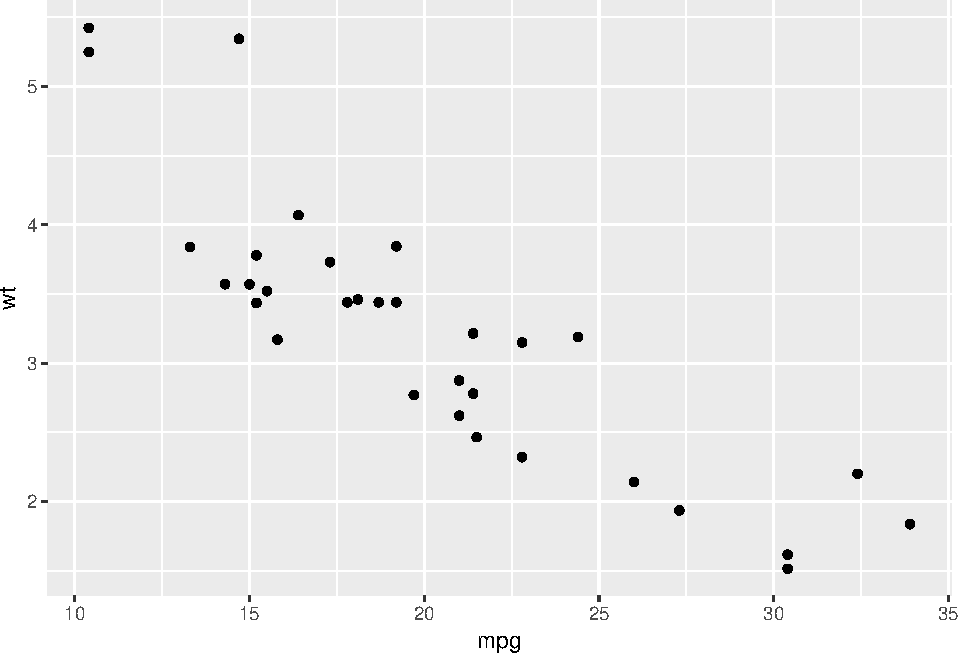
\includegraphics{demo_files/figure-latex/unnamed-chunk-2-1.pdf}

\end{document}
